\documentclass{beamer}

\usepackage{natbib}
\bibliographystyle{plain}
\renewcommand\phi\varphi


\mode<presentation> {

\usetheme{Madrid}

%\setbeamertemplate{footline} % To remove the footer line in all slides uncomment this line
%\setbeamertemplate{footline}[page number] % To replace the footer line in all slides with a simple slide count uncomment this line

%\setbeamertemplate{navigation symbols}{} % To remove the navigation symbols from the bottom of all slides uncomment this line
}

\usepackage{graphicx} % Allows including images
\usepackage{booktabs} % Allows the use of \toprule, \midrule and \bottomrule in tables
\usepackage{tikz}
\usetikzlibrary{bayesnet}

%----------------------------------------------------------------------------------------
%	TITLE PAGE
%----------------------------------------------------------------------------------------

\title[Semantic Frame Induction]{Semantic Frame Induction} % The short title appears at the bottom of every slide, the full title is only on the title page

\author{Eli Drumm, Bill Noble, Jacob Verdegaal} % Your name
\institute[UvA] % Your institution as it will appear on the bottom of every slide, may be shorthand to save space
{
University of Amsterdam \\ % Your institution for the title page
\medskip

}
\date{12/16/14}

\begin{document}

\begin{frame}
\titlepage 
\end{frame}

\begin{frame}
\frametitle{Overview} 
\tableofcontents 
\end{frame}

%----------------------------------------------------------------------------------------
%	PRESENTATION SLIDES
%----------------------------------------------------------------------------------------

%------------------------------------------------
\section{Semantic Frames}
%------------------------------------------------


\begin{frame}
  \frametitle{Semantic Frames}
  \begin{itemize}
  \item Frame semantics -- Charles J. Fillmore (1976).
  \item A semantic frame is ``a description of a type of event, relation, 
  or entity and the participants in it.'' (Framenet)
  \item There is no mapping between frames and verbs.
  \end{itemize}
  An example:\\
  \vspace{10pt}
\begin{tabular}{|l|}
  \hline
  \textit{\small predicate:\normalsize}~~~Transaction\\
  \hline
  \hline
  \textit{\small role 1:\normalsize}~~~ baker\\
  \textit{\small role 2:\normalsize}~~~ Alice\\
  \textit{\small role 3:\normalsize}~~~ bread\\
  \hline
\end{tabular}\\
\vfill
\begin{itemize}
\item Alice buys a bread from the baker
\item The baker sells Alice a bread
  \end{itemize}
\end{frame}

\section{Models}

\begin{frame}
  \frametitle{Google Syntactic-Ngrams}
  \begin{itemize}
  \item A syntactic-ngram is a $k$-word rooted subtree for some sentence. 
  \item Google ngrams come from a corpus of 3.5 million English books.
  \item We trimmed the ``verb args'' dataset to consider only subject-verb-object triples (VSO's).
  \item The dataset contains 1,629,120 unique VSO's with a total of 96,245,401 by count.
  \item In our final results we may only use the most common \%20 of these...
  \end{itemize}

\end{frame}

\begin{frame}
  \frametitle{Model 0 - EM }
  \begin{columns}
  \column{.5\textwidth}
    \begin{figure}
    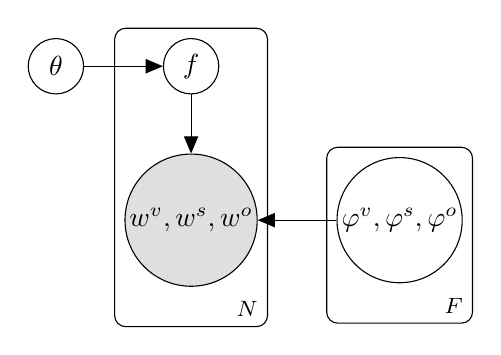
\begin{tikzpicture}
  % Nodes
  \node[obs] (datapoint) {$w^v,w^s,w^o$} ; %
  \node[latent, above=0.75cm of datapoint] (F) {$f$} ; %
  \node[latent, left=of F] (theta) {$\theta$}; %
  \node[latent, right=of datapoint] (phi) {$\varphi^v,\varphi^s,\varphi^o$}; %
  \edge {theta} {F} ; %
  \edge {F} {datapoint}
  \edge {phi} {datapoint} ; %
  \plate {tuples} {(F) (datapoint) } {$N$}; %
  \plate {} {(phi)} {$F$} ; %
\end{tikzpicture}

    \end{figure}
  \column{.5\textwidth} 
  \begin{scriptsize}
  \begin{tabbing}
    $N$ \hspace{10pt}\= number of data points\\
    $F$              \> number of frames\\
    $\theta$         \> distribution over frames\\
    $\varphi_a$      \> distributions (for each frame) over \\ 
                     \> vocabulary of argument $a$\\
    $w_a$            \> datapoint (verb, subject, object)\\
  \end{tabbing}
  \end{scriptsize}
  \end{columns}
\footnotesize{E-Step:}
\[
P(f|w_i) = \frac{\prod_a^{\{v,s,o\}}P(w_i^a|\phi_f^a) P(f|\theta)}{\sum_{f'}^F\prod_a^{\{v,s,o\}}P(w_i^a|\phi_{f'}^a)}
\]
\footnotesize{M-Step:}
\begin{columns}
\column{.5\textwidth}
\[
P(f|\theta) = \frac{\sum_{i=1}^N \mu_i(f)}{\sum_{f'=1}^F\sum_{i=1}^N\mu_i(f')}
\]
\column{.5\textwidth}
\[
P(w|\phi_f^a) = \frac{\sum_{i=1}^N \mu_i(f) C(w,a)}{\sum_{w'=1}^{V^a}\sum_{i=1}^N \mu_i(f) C(w',a)}
\]
\end{columns}
\end{frame}

\begin{frame}
  \begin{columns}
  \column{.5\textwidth}
  \frametitle{Model 1 - Gibbs Sampling}
  \begin{figure}
  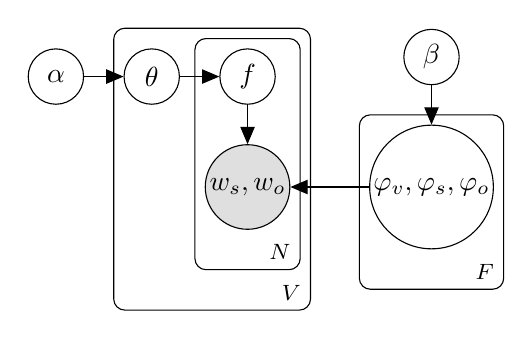
\begin{tikzpicture}[]
    \node[obs]                   (w)     {$w_s,w_o$}; %
    \node[latent, above=0.5cm of w]     (f)     {$f$};
    \node[latent, left=0.5cm of f]     (theta) {$\theta$};
    \node[latent, left=0.5cm of theta] (alpha) {$\alpha$};
    \node[latent, right=of w]    (phi)   {$\varphi_v,\varphi_s,\varphi_o$};
    \node[latent, above=0.5cm of phi] (beta) {$\beta$};
    \edge {alpha} {theta};
    \edge {theta} {f};
    \edge {f} {w};
    \edge {phi} {w};
    \edge {beta} {phi};
    \plate {frames} {(phi)} {$F$};
    \plate {datapoints} {(f) (w)} {$N$};
    \plate {verbs} {(f) (w) (datapoints) (theta)} {$V$};
\end{tikzpicture}

  \end{figure}
  \column{.5\textwidth}
  \begin{scriptsize}
  \begin{tabbing}
    $N$ \hspace{10pt}\= number of data points\\
    $F$              \> number of frames\\
    $V$              \> number of documents (= verb vocabulary)\\
    $\theta$         \> distribution over frames\\
    $\varphi_a$      \> distributions (for each frame) over \\ 
                     \> vocabulary of argument $a$\\
    $w_a$            \> datapoint (verb, subject, object)\\
    $\beta$          \> hyperprior for $\varphi$ (for each argument)\\
    $\alpha$         \> hyperprior for $\theta$ \\
  \end{tabbing}
  \end{scriptsize}
  \end{columns}
\footnotesize{Gibbs:}
\[
P(z_{ij} = f| \mathbf{f}_{-ij},\alpha,\beta,w)
\propto \prod_a^{\{v,s,o\}}\frac{\beta^a + \tilde{C}(f,w_{ij})}{V^a + \tilde{C}(f)}
        \cdot \frac{\alpha + \tilde{C}(i,f)}{F\alpha+\tilde{C}(i)}
\]
\begin{scriptsize}
  \begin{tabbing}
    $\tilde{C}(f,w_{ij})$ \hspace{10pt}\= count times $w_{ij}$ is assigned to frame $f$\\
    $\tilde{C}(f)$                     \> count total data points assigend to $f$\\
    $\tilde{C}(i,f)$                   \> count sentences in document $i$ assigned to $f$\\
    $\tilde{C}(i)$                     \> count sentences in document $i$\\ 
  \end{tabbing}
  \end{scriptsize}

\end{frame}

\section{Results}

\begin{frame}
  \frametitle{Evaluation metrics}
  \begin{itemize}
  \item Frame coherency: for a datapoint $(v,s,o)$ and a tuple $(v^r,s,o)$ where $v^r$ is a random choses verb: $P(v\mid s,o) \geq P(v^r\mid s,o)$  
  \item Frame correctness: for the top 25 most probable verbs per frame $TV$ and framenet classes of verbs $FN$: \[\frac{2|TV\cap FN|}{|TV|+|FN|}\]
  \end{itemize}
\end{frame}

\begin{frame}
  \frametitle{Results EM - model 0}
  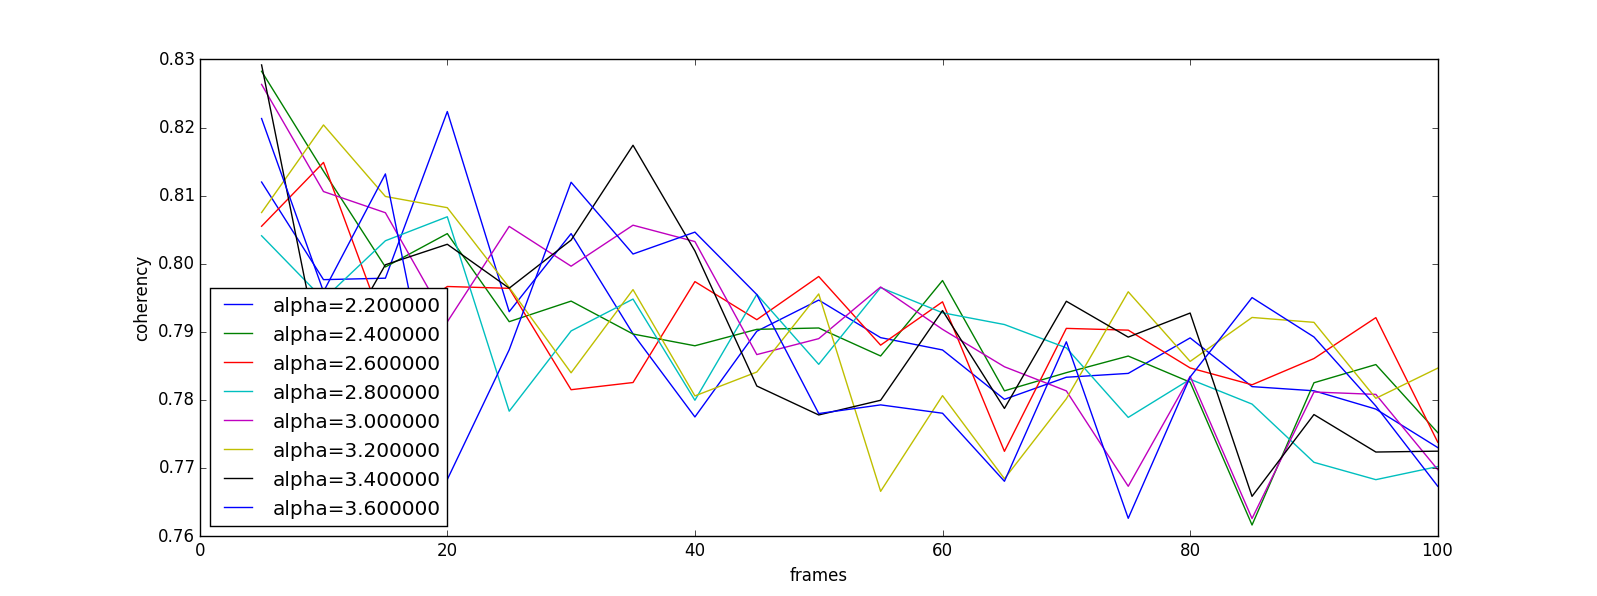
\includegraphics[width=\hsize,height=.4\vsize]{results_1}\\
  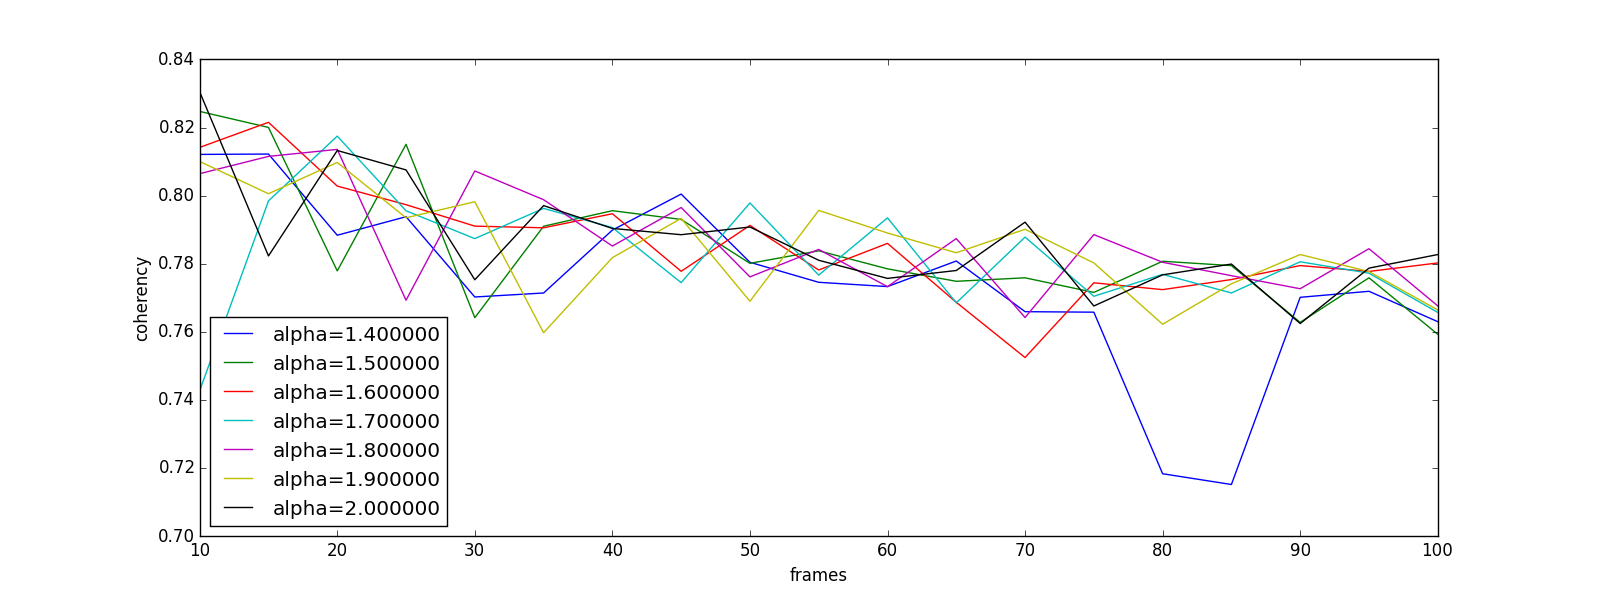
\includegraphics[width=\hsize,height=.4\vsize]{results_2}
\end{frame}

\begin{frame}
  \frametitle{Results Gibbs sampling - model 1}
  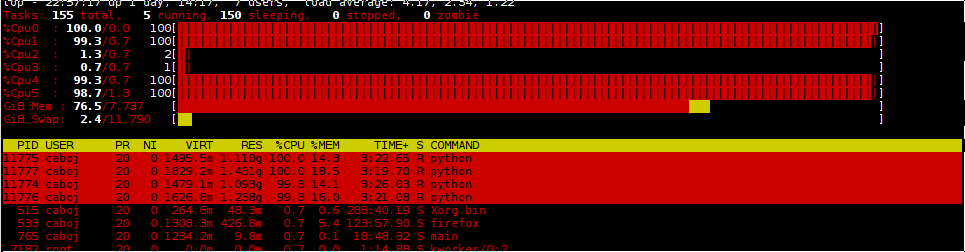
\includegraphics[width=\hsize]{bsy}\\
  
\end{frame}

\section{References}
\begin{frame}[t,allowframebreaks]
\nocite{*}
\bibliography{refs.bib}
\end{frame}




\end{document}
